%---------- Inleiding ---------------------------------------------------------

\section{Introductie}%
\label{sec:introductie}

% Met een jaarlijks budget van 32 miljoen in het vakgebied kunstmatige intelligentie (AI) op de werkvloer is België een pionier \autocite{Crevits2022}.  Zo zijn er verschillende projecten, om taalgerelateerde AI-ontwikkelingen op te starten, uit de grond gestampt. Het amai!-project \footnote{https://amai.vlaanderen/}  verenigt AI-softwarebedrijven uit verschillende domeinen om zo met AI-toepassingen te maken die processen automatiseren om de werkdruk te verminderen, zoals binnen het onderwijs \textit{real-time} ondertiteling en een taalassistent voor leerkrachten in meertalige klasgroepen.

Het Vlaamse middelbaar onderwijs staat nu op barsten, want de leraren en scholieren in het Vlaamse middelbaar onderwijs ondergaan aan de werkdruk en stress. De derde graad in het middelbaar onderwijs is een cruciale stap voor de verdere loopbaan van scholieren, al hebben scholieren moeite met de gekregen vakliteratuur \autocite{Dapaah2022}. Het STEM-agenda\footnote{https://www.vlaanderen.be/publicaties/stem-agenda-2030-stem-competenties-voor-een-toekomst-en-missiegericht-beleid} van de Vlaamse Overheid bestaat uit aandachtspunten om het STEM-onderwijs tegen 2030 aantrekkelijker te maken door de ondersteuning voor zowel leerkrachten als scholieren te verbeteren. Het overbruggen van wetenschappelijke jargon is echter nergens in de aandachtspunten van het STEM-agenda terug te vinden, maar geautomatiseerde en adaptieve tekstvereenvoudiging biedt een revolutionaire oplossing aan. 

Dit onderzoek laat zien hoe de inhoud van wetenschappelijke artikelen op een geautomatiseerde wijze vereenvoudigd kan worden, gericht op de behoeften van scholieren met dyslexie in de derde graad van het middelbaar onderwijs. Hierbij wordt gestart met een theoretische basis voor tekstvereenvoudiging en een literatuurstudie naar de uitdagingen die een toepassing in acht moet nemen. In een vervolgstap wordt met een veldonderzoek gekeken naar bestaande AI-toepassingen voor tekstvereenvoudiging in Nederlandse en Engelse teksten. Hierna beschrijft het onderzoek een pipeline voor geautomatiseerde en adaptieve tekstvereenvoudiging en staat stil bij de verschillende metrieken om de vereenvoudigde tekst te beoordelen. Daarna vindt een vergelijking plaats tussen de vereenvoudigde tekstinhoud van verschillende aangehaalde toepassingen, die beoordeeld wordt met behulp van enquêtes en statistische metrieken. Tot slot worden de resultaten van het onderzoek gebruikt om inzicht te krijgen in hoe wetenschappelijke artikelen op een geautomatiseerde en adaptieve manier vereenvoudigd kunnen worden voor scholieren met dyslexie in het derde graad middelbaar onderwijs. Dit leidt tot verdere ontwikkeling voor AI-ontwikkelaars om een bruikbare toepassing te creëren voor gebruik in het onderwijs.


% Als laatste beschrijving haalt het onderzoek de verschillende evaluatietechnieken aan die nodig zijn om een vereenvoudigde tekst te beoordelen, alsook welke ethische aspecten ontwikkelaars in acht moeten houden bij het opzetten van een dergelijke toepassing. 

%---------- Stand van zaken ---------------------------------------------------

\section{State-of-the-art}%
\label{sec:state-of-the-art}

% Deelvraag: Wat is tekstsimplificatie
De voorbije tien jaar is kunstmatige intelligentie (AI) sterk verder ontwikkeld. De toename in kennis zorgde voor nieuwe toepassingen. Tekstvereenvoudiging vloeide hier uit voort. Momenteel bestaan er al robuuste toepassingen die teksten kunnen vereenvoudigen, zoals Resoomer\footnote{https://resoomer.com/nl/}, Paraphraser\footnote{https://www.paraphraser.io/nl/tekst-samenvatting} en Prepostseo\footnote{https://www.prepostseo.com/tool/nl/text-summarizer}. Binnen het kader van tekstvereenvoudiging is er bestaande documentatie beschikbaar waar onderzoekers het voordeel van toegankelijkheid aanhalen, maar deze toepassingen ontbreken de extra noden die scholieren met dyslexie in het derde graad middelbaar onderwijs vereisen.

Het algemene doel van tekstvereenvoudiging is om ingewikkelde bronnen toegankelijker te maken. Het zorgt voor verkorte teksten zonder de kernboodschap te verliezen. Tekstvereenvoudiging gebeurt doorgaans op één van drie manieren. Er is conceptuele vereenvoudiging waarbij documenten naar een compacter formaat worden getransformeerd. Daarnaast is er uitgebreide modificatie die kernwoorden aanduidt door gebruik van redundantie. Als laatste is er samenvatting die documenten verandert in kortere teksten met alleen de topische zinnen. Met deze concepten zijn ontwikkelaars in staat om ingewikkelde woorden te vervangen door eenvoudigere synoniemen of zinnen te verkorten zodat ze sneller leesbaar zijn \autocite{Siddharthan2014}.

Tekstvereenvoudiging behoort tot de zijtak van natuurlijke taalverwerking (NLP) in kunstmatige intelligentie. NLP omvat methodes om, door machinaal leren, menselijke teksten om te zetten in tekst voor machines. Documenten vereenvoudigen met NLP kan op twee manieren: extract of abstract. Bij extractieve simplificatie worden zinnen gelezen zoals ze zijn neergeschreven. Vervolgens bewaart een document de belangrijkste taalelementen om de tekst te kunnen hervormen. Deze vorm van tekstvereenvoudiging komt het meeste voor \autocite{Sciforce2020}. Daarnaast is er abstracte simplificatie die de kernboodschap van de zin bewaart en daarmee een nieuwe zin opbouwt. Volgens het onderzoek van \textcite{Chowdhary2020} heeft deze vorm potentieel dankzij de menselijke interpretatie, maar zit nog in de kinderschoenen.

% Deelvraag 2: Bewezen voordelen van tekstsimplificatie bij scholieren met dyslexie
Voor kinderen met dyslexie bestaan digitale hulpmiddelen die voor een betere visuele presentatie zorgen van teksten. Zo haalt het onderzoek van \textcite{Rello2012} tips aan waarmee teksten en documenten rekening moeten houden bij scholieren met dyslexie in het derde graad middelbaar onderwijs. Het gaat over speciale lettertypes, spreiding tussen woorden en het gebruik van inzoomen op aparte zinnen. Het onderzoek haalt aan dat teksten voor deze unieke noden aanpassen tijdrovend is, dus tekstvereenvoudiging door kunstmatige intelligentie kan een revolutionaire oplossing bieden. 

Het onderzoek van Franse wetenschappers \newline \textcite{Gala2016} illustreert dat manuele tekstvereenvoudiging schoolteksten toegankelijker \newline maakt voor kinderen met dyslexie. Dit deden ze door simpelere synoniemen en zinsstructuren te gebruiken. Verwijswoorden werden vermeden en woorden kort gehouden. De resultaten waren veelbelovend. Het leestempo lag hoger en de kinderen maakten minder leesfouten. Ook bleek er geen verlies van begrip in de tekst bij geteste kinderen. Resultaten van de studie werden gebundeld voor de mogelijke ontwikkeling van een AI hulpmiddel.

De Universiteit van Kopenhagen is met bovenstaande idee aan de slag gegaan. Onderzoekers \textcite{Bingel2018} hebben gratis software ontwikkeld, genaamd Hero\footnote{https://beta.heroapp.ai/}, om tekstvereenvoudiging voor scholieren in het middelbaar onderwijs met dyslexie te automatiseren. De software bestudeert met welke woorden de gebruiker moeite heeft, en vervangt die door simpelere alternatieven. Hero bevindt zich in beta-vorm en wordt enkel in het Engels en het Deens ondersteund. 

% Deelvraag: Waarop moet er gefixeerd worden bij een wetenschappelijke paper
\textcite{PlavenSigray2017} halen aan hoe onderzoekers in hun taalbubbel blijven, wat gevolgen voor de lezers met zich meebrengt. Daarnaast brengt de stijging aan het gebruik van acroniemen volgens \textcite{Barnett2020} een extra obstakel met zich mee. Het onderzoek van \textcite{Donato2022} wijst uit dat scholieren met dyslexie in het middelbaar onderwijs die uit hun richting vallen, te wijten zijn aan ondoorgrondelijke teksten. Dit bleek vooral bij STEM-richtingen het geval. 

% Deelvraag: Uitdagingen van AI-software met tekstsimplificatie
\textcite{Roldos2020} haalt aan dat NLP in de laatste decennia volop in ontwikkeling is, maar ontwikkelaars botsen nog op uitdagingen. Het gaat om zowel interpretatie- als dataproblemen bij AI machines. Het onderzoek haalt twee punten aan. Allereerst is het voor een machine moeilijk om de context van homoniemen te achterhalen. Bijvoorbeeld bij het woord ‘bank’ is het niet duidelijk voor de machine of het gaat over de geldinstelling of het meubel. Daarnaast zijn synoniemen geen probleem voor tekstverwerking.

Het onderzoek van \textcite{Sciforce2020} haalt aan dat het merendeel van NLP-toepassingen Engelstalige invoer gebruikt. Niet-Engelstalige toepassingen zijn zeldzaam. De opkomst van AI technologieën die twee datasets gebruiken, biedt een oplossing voor dit probleem. De software vertaalt eerst de oorspronkelijke tekst naar de gewenste taal, voordat de tekst wordt herwerkt. Hetzelfde onderzoek bewijst dat het vertalen van gelijkaardige talen, zoals Duits en Nederlands, een minimaal verschil opleverd.

% Deelvraag: Stand van zaken bij Belgische secundaire scholen
De Vlaamse overheid leent gratis abonnementen uit voor voorlees- en schrijfsoftware. De voornaamste zijn SprintPlus\footnote{https://www.sprintplus.be/}, Alinea\footnote{https://sensotec.be/product/alinea-suite/} en Kurzweil3000\footnote{https://sensotec.be/product/kurzweil-3000/}. Vlaamse scholieren met dyslexie in het middelbaar onderwijs kunnen voor deze software een gratis abonnement of licentie aanvragen. Al bieden de vijf softwarepakketten elk een samenvattingsfunctie aan, echter ligt de focus op spreek- en luisterfuncties waarbij het samenvatten en markeren van tekst als extra wordt gehouden.

ChatGPT\footnote{https://chat.openai.com/chat} van OpenAI is een \textit{chatbot} gebouwd op het GPT-3 model. Het GPT-3 model omvat meer dan vijf miljard verschillende woorden, wat het revolutionair maakt voor AI taaltoepassingen. Nadelig moet de \textit{chatbot} via de online toepassing expliciet gevraagd worden om tekst te kunnen vereenvoudigen. \textcite{Verhoeven2023} haalt aan dat toepassingen zoals ChatGPT een wondermiddel zijn om de werklast van routinematig en boilerplate werk te verminderen in het onderwijs. Toepassingen ontwikkelen met het GPT-3 model is mogelijk, al is de API van GPT-3 enkel tegen betaling beschikbaar. Readable\footnote{https://readable.com/} is een Engelstalige AI toepassing dat zinnen beoordeeld met leesbaarheidsformules. Bij beide tools is het enkel mogelijk om tekst op de webpagina te plakken, dus er kunnen geen PDF-documenten of scans worden geüpload en eenzelfde werking verwachten.

Vlaanderen heeft weinig zicht op de geïmplementeerde AI software in scholen. Dit werd vastgesteld door \autocite{Martens2021}, een samenwerking tussen de Vlaamse universiteiten en overheid voor kunstmatige intelligentie. Vergeleken met andere Europese landen, maakt België het minst gebruik van leerling-georiënteerde hulpmiddelen. Degenen die wel gebruikt worden, zijn vooral online leerplatformen voor zelfstandig werken. Ook maakt België amper gebruik van beschikbare software die de leermethoden en -noden van leerlingen evalueert \autocite{Martens2021a}. 

% Deelvraag: Wat is er nodig voor tekstsimplificatie? 
Python staat bovenaan de lijst van programmeertalen voor NLP-toepassingen. Volgens het onderzoek van \textcite{Thangarajah2019} is dit te wijten aan de eenvoudige syntax, kleine leercurve en grote beschikbaarheid van kant-en-klare bibliotheken. Moeilijke wiskundige berekeningen of statistische analyses kunnen worden uitgevoerd door middel van één lijn code. Een artikel van \textcite{Malik2022} haalt de twee meest voorkomende aan, namelijk NLTK\footnote{https://www.nltk.org/} en Spacy\footnote{https://spacy.io/}.

Iedere soort tekstvereenvoudiging omvat verschillende fases. Het onderzoek van \textcite{Shardlow2014} wijst uit dat een pipeline voor lexicale vereenvoudiging uit vier fases bestaat. Een \textit{proof-of-concept} genaamd \textit{Deep Martin}\footnote{https://github.com/chrislemke/deep-martin} bouwt verder op dit theoretisch concept. Hun pipeline maakt gebruik van \textit{custom transformers} om invoertekst om te zetten naar een vereenvoudigde versie van de tekstinhoud.

\textcite{Garbacea2021} benadrukken dat AI ontwikkelaars te weinig aandacht besteden aan de eerste twee stappen van de pipeline voor tekstvereenvoudiging, namelijk het achterhalen waarom een woord of zin moet worden aangepast. Zij halen aan dat de ethische aspecten van AI taaltoepassingen aan de eindgebruiker moet worden meegegeven. Hetzelfde onderzoek haalt twee aspecten aan dat een AI toepassing na een vereenvoudiging moet kunnen aantonen. Allereerst moet de toepassing meegeven waarom een zin of woord is aangepast. De moeilijkheidsgraad van de woord of de zin moet worden bewezen door het model. \textcite{Iavarone2021} haalt zo een methode aan om de moeilijkheidsgraad te bepalen. In dit onderzoek werden regressiemodellen ingezet om een gemiddelde moeilijkheidspercentage te berekenen per zin. Verder haalt \textcite{Garbacea2021} als tweede pijler aan dat de complexe delen van zin gemarkeerd moeten worden. Zij halen \textit{lexical of deep learning} methoden aan waarmee AI ontwikkelaars erin slagen om deze twee fasen in hun AI toepassing te kunnen uitwerken.

Er is een tactvolle aanpak nodig om een vereenvoudigde tekst met AI te beoordelen. De studie van \textcite{Swayamdipta2019} haalt aan dat er extra nood is aan NLP-modellen waarbij de tekst zijn kernboodschap behoudt. Samen met Microsoft Research bouwden ze NLP-modellen die gericht waren op de bewaring van zinsstructuur en -context door \emph{scaffolded learning}. Hiervoor maakten de onderzoekers gebruik van een voorspellingsmethode die de positie van woorden en zinnen in een document beoordeelde. Daarnaast wijst het onderzoek van \textcite{Readable2021} uit dat de Flesch-Kincaid leesbaarheidstest een manier aanbiedt om vereenvoudigde tekstinhoud te beoordelen, zonder de nood van vooraf getrainde modellen. Met de Python-library \textit{textstat}\footnote{https://pypi.org/project/textstat/} kan deze score eenvoudig worden berekend.

\begin{figure}
	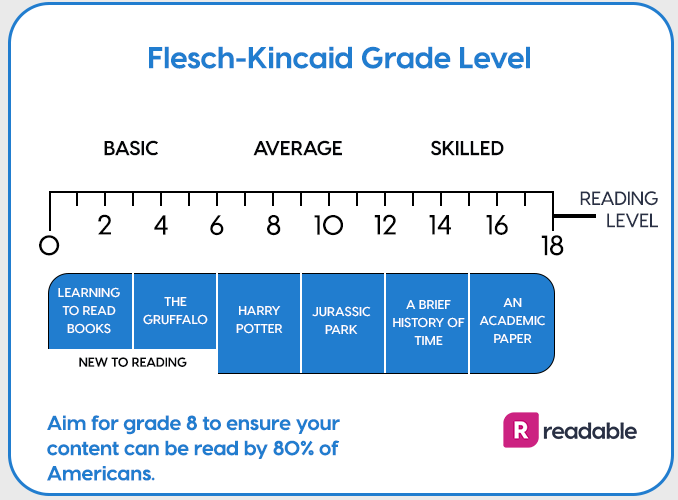
\includegraphics[width=\linewidth]{img/Screenshot_302.png}
	\caption{Afbeelding van \autocite{Readable2021}}
\end{figure}

% Bovendien zijn er kant-en-klare modellen die de complexiteit van tekst kunnen bepalen, hoewel deze beperkt zijn en vooral gericht zijn op Engelse teksten, zoals BERT\footnote{https://huggingface.co/docs/transformers/model\_doc/bert}, XLNet\footnote{https://huggingface.co/docs/transformers/model\_doc/xlnet}, GPT-3\footnote{https://platform.openai.com/docs/} en .

%---------- Methodologie ------------------------------------------------------
\section{Methodologie}%
\label{sec:methodologie}

Er wordt een \textit{mixed-methods} onderzoek uitgevoerd om te bepalen of een AI toepassing de tekstinhoud van een wetenschappelijke paper op maat van de noden voor een scholier met dyslexie in het derde graad middelbaar onderwijs kan vereenvoudigen. Het onderzoek houdt zes fases in. 

De eerste fase is het proces van tekstvereenvoudiging beschrijven, waaronder een omschrijving van het begrip en de verschillende soorten van tekstvereenvoudiging met AI. Dit gebeurt via een grondige studie van vakliteratuur en wetenschappelijke teksten. Ook blogs van experten komen hier aan bod. Na het verwerven van de nodige inzichten wordt er een verklarende tekst opgesteld.

De tweede fase bestaat uit het analyseren van wetenschappelijke werken over de bewezen voordelen van tekstvereenvoudiging bij scholieren met dyslexie van het derde graad middelbaar onderwijs. Hiervoor zijn geringe thesissen beschikbaar, die zorgvuldigheid vragen tijdens interpretatie. De resulterende tekst bevat de voordelen samen met hun wetenschappelijke onderbouwing.

De derde fase is opnieuw een beschrijving. Hier worden de valkuilen bij taalverwerking met AI software nagegaan. Deze fase van het onderzoek brengt mogelijke nadelen en tekortkomingen van AI software bij tekstvereenvoudiging aan het licht. Dit gebeurt aan de hand van een technische uitleg.

De vierde fase omvat een toelichting over beschikbare AI toepassingen voor tekstvereenvoudiging. Aan de hand van een veldonderzoek op het internet en bij bedrijven wordt er op zoek gegaan naar dergelijke software. Er wordt niet gezocht naar vertaalsoftware of toepassingen die de inhoud van een afbeelding of tekstbestand omzet naar tekstinhoud. Het resultaat van deze fase is een longlist van alle beschikbare AI toepassingen die teksten kunnen vereenvoudigen.

De vijfde fase omschrijft de technische uitwerking van een pipeline voor tekstvereenvoudiging, alsook een shortlist van metrieken om de vereenvoudigde tekstinhoud te evalueren. Er zal een tekstvereenvoudigingspipeline worden ontwikkeld met beschikbare kant-en-klare bibliotheken, \textit{transformers} en algoritmen. Het resultaat van deze fase is een pipeline opgebouwd in de programmeertaal Python. 

De zesde fase bestaat uit een toelichting van de beschikbare evaluatiemetrieken om vereenvoudigde tekst te kunnen beoordelen. Het resultaat is een shortlist van alle evaluatiecriteria waaraan de uitvoertekst van een tekstvereenvoudigingstoepassing moet voldoen.

De zevende en laatste fase omvat een vergelijkende studie van de gevonden AI-toepassingen die tekst vereenvoudigen en de pipeline. De tekstinhoud van wetenschappelijke papers die in een derde graad middelbaar onderwijs worden gebruikt, dienen hier als invoertekst voor de evaluatie. De subjectieve test gebeurt aan de hand van een enquête en een \textit{think-aloudtest}. De objectieve testen gebeuren op basis van de shortlist uit de derde fase en de shortlist van metrieken uit de zesde fase. Ten slotte volgt er een persoonlijk advies over de nodige ontwikkelingen in het vak op vlak van Nederlandstalige tekstvereenvoudiging.

%---------- Verwachte resultaten ----------------------------------------------
\section{Verwacht resultaat, conclusie}
\label{sec:verwachte_resultaten}

Er wordt verwacht dat de software, die nu in het onderwijs wordt ingezet, niet voldoet aan de noden van een scholier met dyslexie in het derde graad middelbaar onderwijs. Dit is omdat er onvoldoende rekening wordt gehouden met hun uitdagingen. Bestaande internationale AI-toepassingen bieden een gelijkwaardige oplossing, al steekt ChatGPT met het GPT-3 model boven de rest uit. Met dit model kan er een krachtige applicatie worden opgebouwd. Het vertalen van de vereenvoudigde tekstinhoud bij een internationale AI-toepassing kan afwijken van de oorspronkelijke context.

Er zijn onvoldoende kant-en-klare algoritmen en modellen beschikbaar om een \textit{pipeline} voor tekstvereenvoudiging te bouwen, vooral gericht op scholieren met dyslexie in het middelbaar onderwijs. De vereenvoudigde inhoud uit de \textit{pipeline} voldoet niet aan hun noden. De \textit{pipeline} heeft nood aan \textit{custom transformers} om belovende resultaten te bekomen. Er is nood aan Nederlandstalige \textit{word embeddings} die de complexiteit per woord bijhouden en kant-en-klare modellen die de tekstinhoud van wetenschappelijke papers kunnen vereenvoudigen. Werken met word embeddings uit een Germaanse taal en later de vereenvoudigde tekst vertalen, verlaagt de nauwkeurigheid van het model maar is een aanvaardbaar alternatief.